\chapter{Search Engine}
An \emph{search engine} it comes of several components that can be viewed in figure \ref{img:searchEngine},
we will start talking about crawling and then we will introduce the other components.

In figure \ref{img:bowTie} there is a bow tie that exploits some consideration about crawler where
we can see that web pages that search engine consider are a small amount of all pages. 

\section{Crawling}
Crawling is a graph visit of the web graph, run 24h each days, in order to discover new web pages and we 
have a direct graph $G = (N, E)$ with $N$ that indicate $N$ changes in nodes (usually trillion of nodes) and
$E$ indicate a link between two nodes.

In crawling we have to choose between several issues:
\begin{itemize}
    \item How to crawl? we can choose between quality ("Best" pages first), efficiency (Avoid duplication) and also 
          about malicious pages (Spam pages, Spider traps) including dynamically generated.
    \item How much to crawl and thus index? Coverage and Relative Coverage (coverage comparated with competitor)
    \item How often to crawl? Freshness: How much has changed?
\end{itemize}
Actually is difficult to decide how to implement and design a crawler that should respect the issues that we have
introduced before.

In figure \ref{img:crawler} it is possible to note the general structure of crawler process, in figure \ref{img:crawlerElement} it 
possible to note the component used to implement a crawler and in the end in figure \ref{img:crawlerAlgorithm} there is an pseudocode 
implementation of Crawler's component.

\begin{figure}
    \caption {Diagramm of Crawler operation}
    \label{img:crawler}
    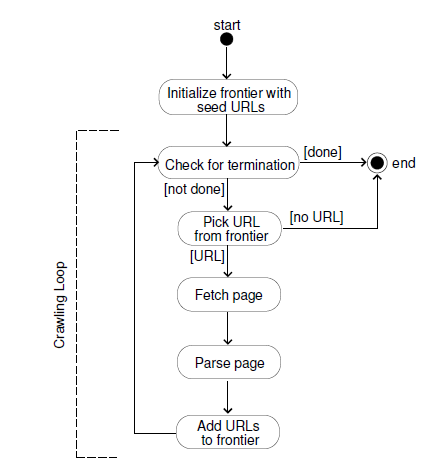
\includegraphics[width=\textwidth]{Images/crawler}
\end{figure}

\begin{figure}
    \caption{Component of Crawler}
    \label{img:crawlerElement}
    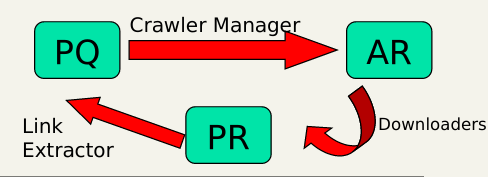
\includegraphics[width=\textwidth]{Images/crawlerComponents}
\end{figure}

\begin{figure}
    \caption{Pseudocode of Crawler components}
    \label{img:crawlerALgorithm}
    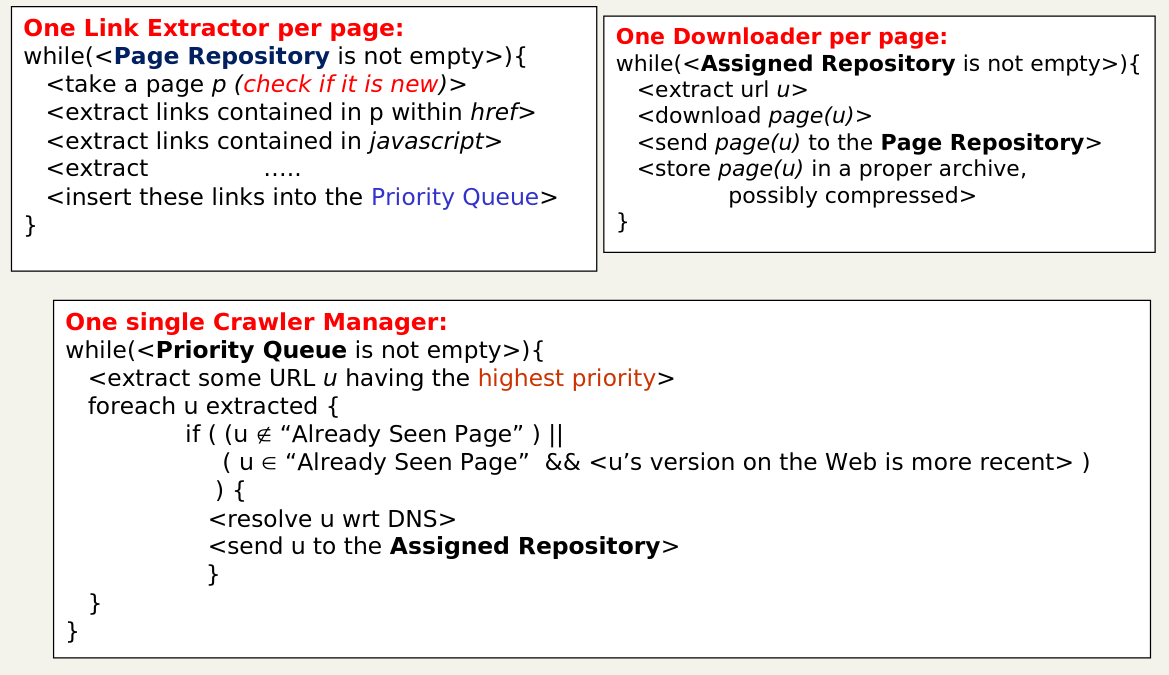
\includegraphics[width=\textwidth]{Images/crawlerPseudocode}
\end{figure}
In visiting the URL frontier we have to define how "good" a page is and there exists several metrics (BFS, DFS, RANDOM, PAGERANK and so on) and also now
we will introduce \emph{Mercator}, an example of search engine released in $1999$, where are present $3$ assumpionts:
\begin{enumerate}
    \item Only one connection per host is open at a time.
    \item a waiting time of a few seconds occurs between successive requests to the same host.
    \item high-priority pages are crawled preferentially.
\end{enumerate}
The structure of Mercator can be viewed in figure \ref{img:mercator} and we have that \emph{Front queues} manage prioritization: prioritizer assigns to an URL an integer priority (refresh,
quality, application specific) between $1$ and $K$ and appends URL to corresponding queue, according to priority.\newline
\emph{Back queues} enforce politeness: each back queue is kept non-empty and contains only URLs from a single host; in a back-queue request it select a front queue randomly, biasing towards higher queues.

\begin{figure}
    \caption{Structure of Mercator search engine}
    \label{img:mercator}
    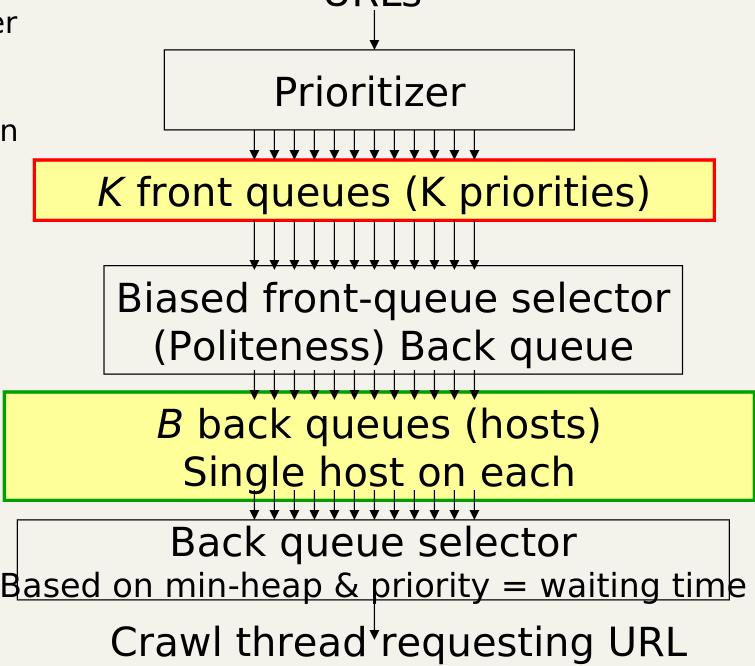
\includegraphics[width=\textwidth]{Images/mercator}
\end{figure}
The \emph{min-heap} contains one entry per back queue and the entry is the earliest time $t_e$ at which the host corresponding to the back queue can be “hit again”:
this earliest time is determined from last access to that host and any time buffer heuristic we choose.\newline
The \emph{crawl thread} consist that a crawler seeks a URL to crawl: extracts the root of the heap, waits the indicate time $t_{url}$, parses URL and adds its out-links to the Front queues.\newline
If back queue $q$ gets empty, pulls a URL $v$ from some front queue (more prob for higher queues): if there’s already a back queue for v’s host, append v to it and 
repeat until q gets not empty, else make q the back queue for v’s host.\newline
If back queue q is non-empty, pick URL and add it to the min-heap with $priority = waiting time t_{url}$.

To check if the page has been parsed/downloaded before URL match, duplicate document match and near-duplicate document match we have several solutions:
\begin{itemize}
    \item Hashing on URLs: after $50$ bln pages, we have “seen” over $500$ bln URLs and each URL is at least $1000$ bytes on average so in overall we have about $500.000 Tb (=500 Pb)$ for just the URLS
    \item Disk access with caching (e.g. Altavista): $>5$ ms per URL check and $>5 ms * 5 * 10^{11}$ URL-checks ($80 years/1PC$ or $30gg/1000 PCs$).
    \item \emph{Bloom Filter} (Archive): for $500$ bln URLs we have about $500 Tbit = 50Tb$
\end{itemize}

\section{Bloom Filter}
    Bloom Filter consist to create a binary array $B[1, m]$ 
 Consider a family of k hash functions that map a
key (URL) to a position (integer) in B

\subsection{Spectral Bloom Filter}
    We define now an evolution of Bloom Filter, used not only in URL match, with the following definition
    \begin{defi}[Spectral Bloom Filter]
         We have a multiset $M = (S, f_X)$ where $S$ is a multiset and $f_X$ is a count function that return the number of occurrences of $x$ in $M$
    \end{defi}
    Comparated with Bloom Filter we have an slightly large usage of space, but we achieve better performance, and also can be built incrementally for streaming data.

    Applications of this data structure is to answer to two common query:
    \begin{description}
        \item [Iceberg query: ] given $x$ check if $f_X > T$, where $T$ is a dynamically threshold
	\item [Aggregate query: ] $SELECT count(a1) FROM R WHERE a1 = v$
    \end{description}
    B vector is replaced by a vector of counters $C_1, C_2, \dots, C_m$, where $C_i$ is the sum of $f_X$ values for elements $x \in S$ mapping to $i$, and approximations of $f_X$ are stored 
    into $C_{h_1(x)}, C_{h_2(x)}, \dots, C_{h_k(x)}$, but due to conflicts $C_i$ provide only an approximation.

    In figure \ref{img:approximation} is possible to note what is good approximation or a bad approximation of $f_X$, and insertion and deletion are quite simple because we have only
    to increase/decrease each counter by $1$, instead the search operation return the minimum selection (MS) value defined as 
    \[ m_X = \min \{C_{h_1(x)}, \dots, C_{h_k(x)}\} \]

    \begin{figure}
	\caption{Example of approximation between $C_i$ and $f_X$}
	\label{img:approximation}
	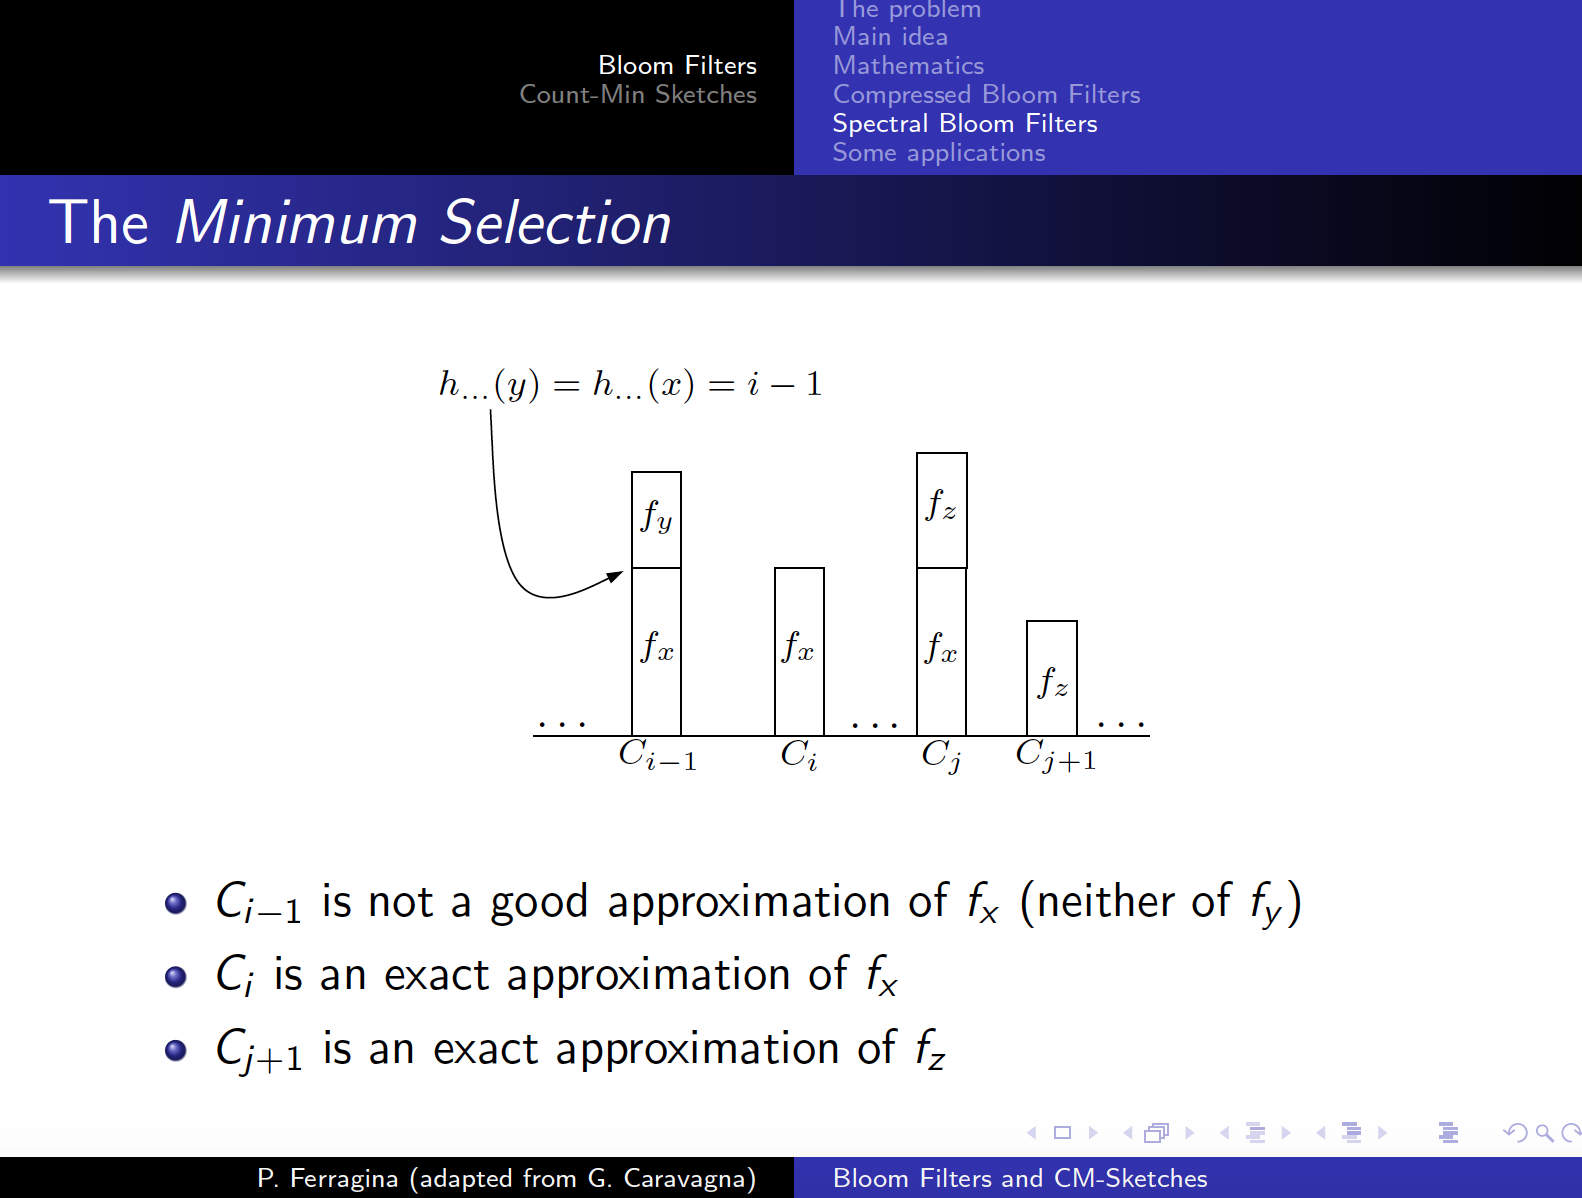
\includegraphics[width=\textwidth]{Images/approximation}
    \end{figure}

    The error rate is the same as bloom filter and we will now prove it 
    \begin{thm}
	For all $x$ it is $f_X \leq m_X$ and we have $f_X \neq m_X$ with probability $E_{SBF} = \epsilon \sim (1-p)^k$
    \end{thm}
    \begin{proof}
	The case that $m_X < f_X$ can not even happen instead the case $m_X > f_X$ happen when all the counter have a collision, that correspond to the event of a false positive in Bloom Filter
    \end{proof}
    Mainly we have two challenges: allow insertion/deletion while we keeping low $E_{SBF}$ and dynamic array of variable-length counters and to solve the first problem we will use \emph{Recurring Minimum (RM)} that is defined as 
    \begin{defi}
	An element has a RM iff more than one of its counters has value equal to the minimum
    \end{defi}
    An item which is subject to a Bloom Error is typically less likely to have recurring minimum among its counters, because we have the following basic idea, using two SBF:
    \begin{enumerate}
	\item For item $x$ with RM we use $m_X$ as estimator, which is highly probable to be correct and hence $E_{SBF_1} < \epsilon$
	\item For items with a SM we use a secondary SBF which is $|SBF_2| << |SBF_1|$ and thus can guarantee $E_{SBF_2} << \epsilon$.
    \end{enumerate}
    With this approach we use more space which could be used for enlarging the single BF, but experiments show that improvements may be remarkable.

    The insertion handles potential future errors, because we increase all counters of $x$ in $SBF_1$ and if $x$ has a $SM$ in $SBF_1$ we look for $x$ in $SBF_2$ and 
    if yes we increase all counters of $x$ in $SBF_2$, otherwise we set $x$ in $SBF_2$ to be the minimum value in $SBF_1$.

    The deletion is the inverse of insertion, so we decrease all counters of $x$ in $SBF_1$ and if $x$ has a SM in $SBF_1$ we decrease all counters of $x$ in $SBF_2$.

    In lookup we have that if $x$ has a RM in $SBF_1$ we return it otherwise we set $m_x^2$ as the value of $x$ in $SBF_2$ that if it is $> 0$ we return it otherwise we return the min value of $x$ in $SBF_1$.


\section{Parallel Crawlers}
    Web is too big to be crawled by a single crawler, work should be divided avoiding duplication so we need several crawlers that works in parallel and assignment 
    between different crawlers can be done in two ways:
    \begin{description}
	    \item [Dynamic assignment: ] central coordinator dynamically assigns URLs to crawlers and it needs communication between coordinator/crawl threads.
	    \item [Static assignment: ] web is statically partitioned and assigned to crawlers and crawler only crawls its part of the web, no need of coordinator and thus communication
    \end{description}
    The Dynamic assignment is problematic because it is computationally expensive and may be complicated, anyway also static assignment has two problem:
    \begin{itemize}
	\item Load balancing the number of URL assigned to crawler because static schemas based on hosts may fail and dynamic assignment may be complicated
	\item Managing the fault-tolerance so in case we have a death of crawler or we have a new crawler we have to recompete the hash function and choose which crawler to assign.
    \end{itemize}
    A nice technique to solve this problem consist in \emph{consistent hashing}, a tool for Spidering, Web Cache, P2P, Routers Load Balance and Distributed FS.\newline
    It consist that item and servers are mapped to unit circle via hash function ID() and item $K$ are assigned to first server $N$ such that $ID(N) \geq ID(K)$, as we can 
    see in figure \ref{img:consistentHashing}.\newline
    Each server gets replicated $\log S$ times, adding a new server moves points between an old server to the new one, only, we have that in average a server gets $\frac{n}{s}$ element.

    \begin{figure}
	\caption{Consistent Hashing Example}
	\label{img:consistenHashing}
	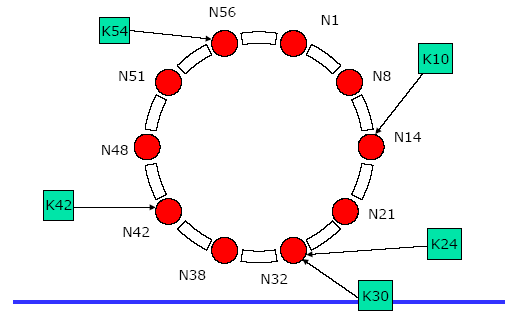
\includegraphics[width=\textwidth]{Images/consistentHashing}
    \end{figure}


\section{Compressed storage of Web Graph}
    Given a directed graph $G = (V, E)$, where $V$ are URLs and $E = (u, v)$ if $u$ has an hyperlink to $v$, also isolated URLs are ignored (they do not have IN and/or OUT)
    and we have three key properties:
    \begin{description}
	    \item [Skewed distribution: ] probability that a node has $x$ links is $1/x^{\alpha}$ with $\alpha \approx 2.1$, so in-value degree follows power law distribution, 
		    			  as we can see in figure \ref{img:altavistaCrawl} and \ref{img:webbaseCrawl}.

					  \begin{figure}
						  \caption{In-degree value in Altavista Crawl in 1997}
						  \label{img:altavistaCrawl}
						  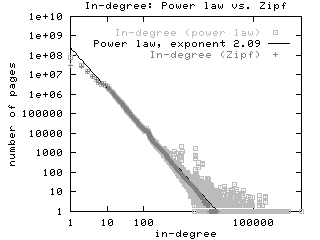
\includegraphics[width=\textwidth]{Images/altavistaCrawl}
					  \end{figure}

					  \begin{figure}
						  \caption{In-degree value in WebBase crawl in 2001}
						  \label{img:webbaseCrawl}
						  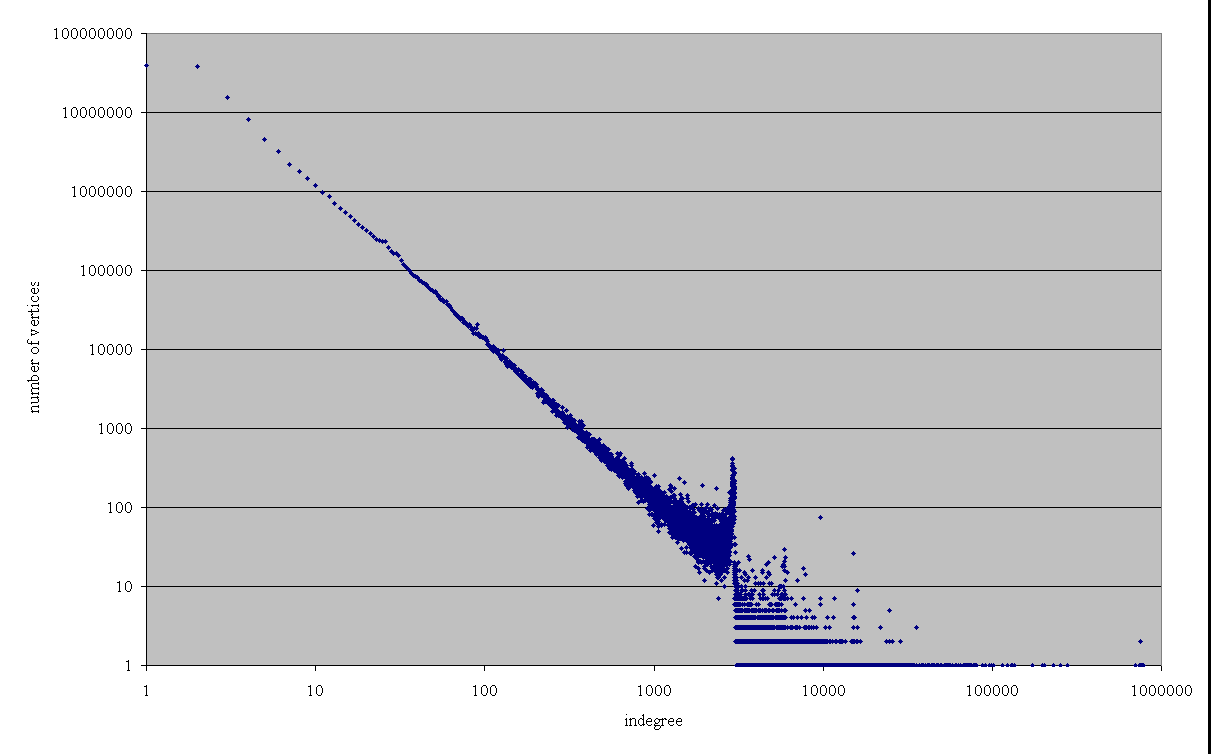
\includegraphics[width=\textwidth]{Images/webBaseCrawl}
					  \end{figure}
						  
	    \item [Locality: ] usually, most of the hyperlinks from URL $u$ point to other URLs that are in the same host of $u$ (about $80\%$), so hosts in the same domain are 
		               close to each other in the lexicographically sorted order, and thus they get close docIDs.

	    \item [Similarity: ] if URLs $u$ and $v$ are close in lexicographic order, then they tend to share many hyperlinks, so we have that each bit of the copy list informs 
		                 whether the corresponding successor of $y$ is also a successor of the reference $x$ and the reference index is the one in $[0, W]$ that gives the best compression,
				 as we can see in figure \ref{img:copyList}.

				 \begin{figure}
					\caption{Example of Copy List}
					\label{img:copyList}
					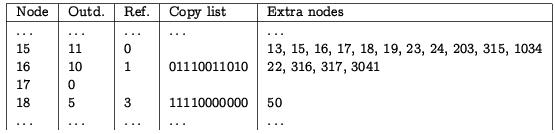
\includegraphics[width=\textwidth]{Images/compressedAdjancency}
				 \end{figure} 
    \end{description}
    To consider these properties we now introduce \emph{copy lists}, to compress information and exploits locality and similarity, but also consider the \emph{copy block}, 
    visible in figure \ref{img:copyBlock}, where the first bit specifies the first copy block and last block is omitted because we know the length from $Out_d$.

    \begin{figure}
	\caption{Example of Copy Block}
	\label{img:copyBlock}
	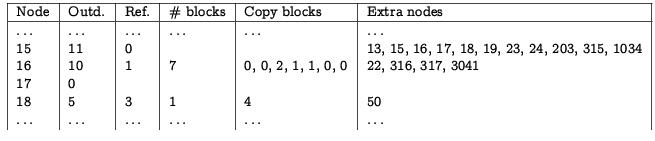
\includegraphics[width=\textwidth]{Images/copyBlock}
    \end{figure}

\section{Locality-sensitive hashing and its applications}
    Given $U$ users, described with a set of d features, the goal is to find (the largest) group of similar users, and to find these group we have three approaches:
    \begin{enumerate}
	\item Try all groups of users and, for each group, check the (average) similarity among all its users.\newline
	      The problem of this approach is that it requires $2^U * U^2$ and also if we limit groups to have a size $\leq L$ we have anyway $U^L * L^2$ 
	      that is computationally infeasible with large $U$.

	\item Interpret every user as a point in a $d$-dim space, and then apply a clustering algorithm, where each iterations require $K * U$ and iterations are relatively small.\newline
	      This approach is locally optimal, comparing users/points costs $O(d)$ in time and space and iterate $k = 1, \dots, U$ costs $U^3 < U^L$, that are in order of years, so 
	      in $T$ time we can manage $U = T^{1/3}$ users.
	
	\item Generate a fingerprint for every user that is much shorter than d and allows to transform similarity into equality of fingerprints.\newline
	      It is randomized, correct with high probability and it guarantees local access to data, which is good for speed in disk/distributed setting
    \end{enumerate}

